% Chapter Template
\newcommand{\drawkey}[3]{
    \draw[line width=0.07cm, draw=#2] (#1) circle [radius=0.15cm];
    \draw[line width=0.07cm, draw=#2] (#1 -0.15) -- ++(0,-0.4);
    \draw[line width=0.07cm, draw=#2] (#1 -0.35) -- ++(-0.2,0);
    \draw[line width=0.07cm, draw=#2] (#1 -0.51) -- ++(-0.2,0);
    \node[below, text=#2] at (#1 -0.6) {#3}
}

% Definizione del comando per disegnare la parentesi
\newcommand{\drawcurlybrace}[3]{% posizione finale, posizione iniziale, testo sopra
    \draw [decorate,decoration={brace,amplitude=10pt,mirror},xshift=-4pt,yshift=0pt]
    (#1) -- (#2) node [black,midway,xshift=-2cm] {};
}

\chapter{Fondamenti di Comunicazioni Sicure}
\label{Capitolo 2} 

In questo capitolo andiamo a trattare quelle che sono le problematiche riguardanti le comunicazioni sicure.
E' possibile realizzare comunicazioni sicure grazie a quelli che cono i crittosistemi, andiamo a vedere come questi vengono utilizzati nelle reti 
di computer per garantire la sicurezza delle comunicazioni.

\section{Teoria}

La comunità scientifica e la storia della crittografia, in questo sezione diamo una panoramica e una descrizione matematica di quelli che sono gli strumenti 
che permettono di rendere le comunicazione sicure. In particolare andiamo a vedere su quali fondamenta questi basano la loro sicurezza.

\subsection{Hash Function}

Una funzione \textbf{hash crittografiche} è una funzione matematica che prende in input un messaggio di lunghezza arbitraria e restituisce un output di
lunghezza fissa, noto come digest.

\begin{equation}
    H: \{0,1\}^*  \to \{0,1\}^n
\end{equation}

\begin{itemize}
    \item $\{0,1\}^*$: rappresenta l'insieme di tutte le stringhe binarie di lunghezza arbitraria.
    \item $\{0,1\}^n$: rappresenta l'insieme delle stringhe binarie di lunghezza fissa $n$.
\end{itemize}

\begin{figure}[h!]
    \centering
    \begin{tikzpicture}[scale=1.5, every node/.style={scale=1}]
        
        % Input message 
        \node[draw, minimum width=3cm, minimum height=1cm, align=center] (input) {Messaggio \\ $m \in \{0,1\}^*$};
        % Hash function box 
        %\filldraw[draw=black, fill=blue!30, rotate=270] (4,0) -- (6,0) -- (5.5,1) -- (4.5,1) -- cycle; 
        \node[draw, minimum width=3cm, minimum height=1cm, align=center, right=2cm of input] (hash) {Funzione di Hash \\ $H$};
        % Digest (output) 
        \node[draw, minimum width=3cm, minimum height=1cm, align=center, right=2cm of hash] (output) {Digest \\  $H(m) \in \{0,1\}^n$};
        % Arrows 
        \draw[->, thick] (input) -- (hash) node[midway, above] {Input};
        \draw[->, thick] (hash) -- (output) node[midway, above] {Output};
        
        % Labels for security properties 
    \end{tikzpicture}
\end{figure}

\vspace{0.2cm}
\noindent
Le proprietà principali che sono richieste ad una funzione di questo dipo sono: 
\begin{itemize}
    \item devono essere progettate in modo tale che sia computazionalmente impraticabile invertire il processo detta anche \textbf{proprietà alle collisioni}, 
    \item una leggere variazione dell'input deve produrre un hash completamente diverso detta anche \textbf{proprietà di diffusione}.
\end{itemize}

Le funzioni di hash crittografiche sono utilizzate in molti contesti, tra cui: verifica di integrità, firma digitale e autenticazione.
Le funzioni di hash sono utilizzate per creare codici di autenticazione dei
messaggi (MAC) per garantire l'integrità e l'autenticità.

\subsection{Schemi crittografici}
Uno schema di cifratura è un insieme di algoritmi e funzioni che definisce come trasformare un messaggio in chiaro (plaintext) in un messaggio cifrato (ciphertext) e viceversa, al fine di garantire la confidenzialità e la sicurezza delle comunicazioni.
Formalmente possiamo rappresentarlo come una quintupla: 

\begin{center}
    \((\mathcal{P}, \mathcal{C}, \mathcal{K}, E, D)\)
\end{center}

\begin{itemize}
    \item \(\mathcal{P}\): Insieme dei messaggi in chiaro (plaintext).
    \item \(\mathcal{C}\): Insieme dei messaggi cifrati (ciphertext).
    \item \(\mathcal{K}\): Insieme delle chiavi utilizzate per la cifratura e decifratura,\textit{key space}.
    \item \(E: \mathcal{K} \times \mathcal{P} \to \mathcal{C}\): Funzione di cifratura.
    \item \(D: \mathcal{K} \times \mathcal{C} \to \mathcal{P}\): Funzione di decifratura.
\end{itemize}

\noindent
Deve esistere una relazione inversa tra le operazioni di cifratura e decifratura:
\begin{equation}
D(k, E(k, m)) = m \quad \forall m \in \mathcal{P}, \, k \in \mathcal{K}
\end{equation}

\begin{figure}[h!]
    \centering
    \begin{tikzpicture}[scale=1.5, every node/.style={scale=1}] 
    % Plaintext
    \node[draw, minimum width=3cm, minimum height=1cm, align=center] (plaintext) {Plaintext\\ $m \in M$};
    % Encryption box 
    \node[draw, minimum width=3cm, minimum height=1cm, below=1cm of plaintext, align=center] (enc) {Cifratura \\ $C = E(K_1,m)$};
    % Ciphertext 
    % se si riesce aggiungere delle linee di delimitazione che facciano intendere che in quesot modo il messaggio è protetto
    \node[draw, minimum width=3cm, minimum height=1cm, right=2cm of enc, align=center] (ciphertext) {Chiphertext\\ $c \in C$};
    % Decryption box 
    \node[draw, minimum width=3cm, minimum height=1cm, right=2cm of ciphertext, align=center] (dec) {Decifratura \\ $M = D(K_2,c)$};
    % Recovered message 
    \node[draw, minimum width=3cm, minimum height=1cm, above=1cm of dec, align=center] (plaintext2) {Plaintext\\ $m \in M$};
    
    % Arrows connecting the elements 
    \draw[->, thick] (plaintext) -- (enc) node[midway, above] {}; 
    \draw[->, thick] (enc) -- (ciphertext) node[midway, above] {}; 
    \draw[->, thick] (ciphertext) -- (dec) node[midway, above] {}; 
    \draw[->, thick] (dec) -- (plaintext2) node[midway, above] {};
    
    % Keys used for encryption and decryption 
    \drawkey{0,-2.1}{black}{$K_1$};
    \drawkey{6.8,-2.1}{black}{$K_2$};
    \end{tikzpicture}
    \label{fig:schema}
    \caption{Funzionamento di uno schema crittografico}
\end{figure}

\noindent
Lo schemo è descirtto in \textit{Fig. \ref{fig:schema}}, ed ha una defizione generale. Però se:
\begin{itemize}
    \item $K_1 = K_2$ allora si parla di un schema di crittografia simmetrico.
    \item $K_1 \neq K_2$ allora si parla di schema di crittografia asimmetrico.
\end{itemize}

\subsubsection{Simmetrici}

Come descritto poco fa, in uno schema simmetrico si utilizza la stessa chiave sia per le operazioni di cifratura che di decifratura. 
Significa che le due parti coinvolte nella comunicazione, devono possedere la stessa chiave segreta (PSK).\\
Gli utilizzi principali prevedono la cifratura dei dati, dato che è molto veloce, e in combinazione con funzioni di hash consente di ottenere codici HMAC

Alcuni esempi di crittosistemi simmetrici sono DES, AES,...



\subsubsection{Asimmetrici}

In uno schema di cifratura asimmetrica, detto anche a \textbf{chiave pubblica}, vengono utilizzate due chiavi distinte: una chiave pubblica e una chiave privata.
Lo spazio delle chiavi \(\mathcal{K}\) è costituito da una coppia di chiavi \((k_{\text{pub}}, k_{\text{priv}})\), dove:

\begin{itemize}
    \item \(k_{\text{pub}}\) è la chiave pubblica (usata per cifrare) 
    \item \(k_{\text{priv}}\) è la chiave privata (usata per decifrare)    
\end{itemize}

\noindent
Le due chiavi sono matematicamente legate, ma è computazionalmente difficile ottenere la chiave privata a partire da quella pubblica (questa è la base della sicurezza).
Quindi le due funzioni si riscrivono come:

\begin{equation}
    E: \mathcal{K}_{\text{pub}} \times \mathcal{P} \to \mathcal{C}
\end{equation}
\begin{equation}
    D: \mathcal{K}_{\text{priv}} \times \mathcal{C} \to \mathcal{P}
\end{equation}

Oltre alla classica cifratura, questa tipologia di schemi consente di realizzare due funzioni importanti, quello \textbf{firma digitale} e di \textbf{scambio di chiave}

Descrivere cosa è una firma, in particolare quella nel caso digitale e come viene utilizzata in combinazione con le funzione di hash per fare hash and sign\\

Oltre a questo poi parlare dello scambio di chiave ovvero l'utilizzo di crittografia asimmetrica per derivare un segreto condiviso tra le due parti.



\begin{figure}[htbp]
    \centering
    \begin{tikzpicture}[node distance=1.5cm]
        \node (entity1) [draw=green, rectangle] {Alice};
        \drawkey{-0.8, -0.8}{black}{$K_{pri}$};
        \drawkey{-1.6, -0.8}{black}{$K_{pub}$};
        \node (entity2) [draw=blue, rectangle, right=of entity1, xshift=3cm] {Bob};
        \draw (entity1) -- ++(0,-5) coordinate (vertical1);
        \draw (entity2) -- ++(0,-5);
        \draw[-stealth] (entity1) ++(0,-1) -- (entity2 |-,-1) node[midway, above, text=black, font=\footnotesize] {$K_{pub}$};
        \draw[stealth-] (entity2) ++(0,-2) -- (entity1 |-,-2) node[midway, above, text=black, font=\footnotesize] {$E(K_{pub},m)$};
    \end{tikzpicture}
    \label{}
    \caption{}
\end{figure}

\subsection{Confronto}

L'assunto che si è fatto in entrambi le tipologie di schema è che l'altra parte della comunicazione avesse ottenuto in qualche modo la chiave. Tuttavia la distribuzione
delle chiavi è un problema importante per il crittosistema ed ognuno ha le proprie caratteristiche. \\

\noindent
Se consideriamo le chiavi simmetriche abbiamo che all'aumentare degli host che vogliamo far comunicare ho bisogno di $n(n-1)/2$ chiavi, dove $n$ è il numero di terminali. Questo approccio è più robusto 
ma come possiamo vedere in \textit{Fig. \ref{fig:chiavi-simmetriche}} il problema porta ad un'esplosione combinatoria. Per questo motivo un approccio che limita questo 
fenomeno è quello del Key Distribution Center (KDC), che tuttavia rappresenta un'approccio centralizzato.
\begin{figure}
    \centering
    \begin{tikzpicture}[font=\sffamily,pics/cgram/.style={code={ \foreach \XX
        [count=\YY starting from 0] in {1,...,#1}
        {\pgfmathsetmacro{\mycolor}{{\LstCols}[\YY]} \node[circle,draw,minimum size=2.
        5em,fill=\mycolor] (c-#1-\XX) at ({{\LstAngles}[#1-2]-\YY*360/#1}:1.5)
        {\setcounter{pft}{\XX}\Alph{pft}};} \foreach \XX [evaluate=\XX as \Ymax using
        {int(\XX-1)}] in {2,...,#1} {\foreach \YY in {1,...,\Ymax}
        {\pgfmathsetmacro{\mycolorA}{{\LstCols}[\XX-1]}
        \pgfmathsetmacro{\mycolorB}{{\LstCols}[\YY-1]} \path (c-#1-\XX) -- (c-#1-\YY)
        coordinate[pos=0.1] (aux0) coordinate[pos=0.9] (aux1); \fill[black] (aux0)
        to[bend left=2] (aux1) to[bend left=2] (aux0); \draw[{Stealth[fill=\mycolorB,
        length=7pt,inset=2pt]}-{Stealth[fill=\mycolorA,length=7pt,inset=2pt]}]
        (c-#1-\XX) -- (c-#1-\YY); }}}}] \def\LstCols{"red","orange","yellow","green!70!
        black","blue!70!white","purple!80!white"} \def\LstAngles{180,150,135,128,150}
        \path (-5,0) pic {cgram=2} (0,0.5) pic {cgram=4} (5,0.5) pic {cgram=6}; 
    \end{tikzpicture}
    \label{fig:chiavi-simmetriche}
    \caption{Distribuzione delle chiavi simmetriche}
\end{figure}

Se invece andiao a considerare i crittosistemi a chiave pubblica abbiamo che questi si possono distribuire tramite certificati di chiave pubblica.
Questi tuttavia hanno bisogno di un'infrastruttura che li sorregge, questa è la PKI (Public Key Infrastructure).
Descrivere quelli che sono i componenti dell'infrastruttura e lo standard per la definzione dei certificati.

\subsection{Sicurezza}

Il \textbf{security level} è una misura della forza che una primitiva crittografica raggiunge rispetto ad attacchi.
Solitamente viene espresso come un numero di “bit di sicurezza”, dove $n$-bit di sicurezza significa che l'attaccante dovrebbe eseguire $2*n$ operazioni per romperlo.

Per i cifrari simmetrici, il \textit{livello di sicurezza} è pari alla dimensione del key-space. Mentre la sicurezza degli algoritmi asimmetrici si basa su problemi matematici che sono efficienti da calcolare in una direzione, ma inefficienti da invertire da parte dell'attaccante.
Tuttavia, gli attacchi contro gli attuali sistemi a chiave pubblica sono sempre più veloci della ricerca a forza bruta dello spazio delle chiavi.

Il NIST (National Institute of Standards and Technology) ha introdotto livelli di sicurezza per gli algoritmi di cifratura asimmetrica e post-quantistica come parte della sua iniziativa per standardizzare algoritmi che resistano anche ai computer quantistici.
I livelli sono definiti in \textit{Tabella \ref{tab:security-levels}}.

% NIST Security Level Table
\renewcommand{\arraystretch}{1.3} 
\begin{table}[ht]
    \centering
    \begin{tabular}{>{\centering\arraybackslash}m{3cm}p{10cm}}
        \hline
        \textbf{Security Level} & \textbf{Descrizione} \\
        \hline
        \textbf{Livello 1} & Sicurezza equivalente alla cifratura simmetrica con chiavi da 128 bit, come AES-128.\\
        \textbf{Livello 2} & Sicurezza equivalente ad attacchi contro SHA-256, con complessità circa pari a 128 bit. Leggermente più sicuro del livello 1. \\
        \textbf{Livello 3} & Sicurezza equivalente alla cifratura simmetrica con chiavi da 192 bit, come AES-192. \\
        \textbf{Livello 4} & Sicurezza equivalente ad attacchi contro SHA-384. Leggermente più sicuro del Livello 3. \\
        \textbf{Livello 5} & Sicurezza equivalente alla cifratura simmetrica con chiavi da 256 bit, come AES-256. \\
        \hline
    \end{tabular}
    \caption{Security Levels definiti dal NIST}
    \label{tab:security-levels}
\end{table}

\newpage
\section{Applicazioni}

Per loro natura le reti sono un mezzo di comunicazione non sicuro, essendo di tipo broadcast.
Nel contesto delle comunicazioni digitali, la crittografia gioca un ruolo fondamentale per garantire la sicurezza dei dati scambiati tra entità remote. 
I crittosistemi, ovvero applicazioni crittografica, combinano algoritmi di cifratura, autenticazione e gestione delle chiavi per garantire la riservetezza e l'integrità dei dati scambiati. 
Uno dei principali modelli di riferimento per la trasmissione di dati su Internet è il modello TCP/IP, che suddivide il processo di comunicazione in diversi livelli, ciascuno con funzioni specifiche.

% MODELLO TCP/IP
\begin{figure}[h!]
    \centering
    \includegraphics[scale=0.3]{Figures/security_tcp.png}
    \label{fig:tcpip}
    \caption{Modello TCP/IP con Protocolli di Sicurezza}
\end{figure}

Come mstrato in \textit{Fig. \ref{fig:tcpip}} possiamo fare sicurezza ai vari livelli della pila, ognuno con le proprie caratteristiche.
Tuttavia fare sicurezza a L3 ha il significativo vantaggio che tutti gli strati superiori convergono su di lui e dunque non è necessario andare a modifcare le singole applicazioni.
IPsec è una suite di protocolli i cui principali componenti, come mostrato in \textit{Fig. \ref{fig:ipsec-suite}}, sono: 

\begin{itemize}
    \item \textbf{AH}: Authentication Header, serve per avere integrità e autenticazione
    \item \textbf{ESP}: Encapsulating Security Payload, permette di rispettare tutti i requisiti di sicurezza
    \item \textbf{SA}: Security Association, è un insieme di parametri che definisce come i dati devono essere protetti durante la comunicazione tra due entità su una rete. Ogni SA contiene le informazioni necessarie per stabilire e mantenere una connessione sicura.
    \item \textbf{Algoritmi}: gli algoritmi crittografici e di hashing ausiliari per ottenere sicurezza
    \item \textbf{IKE}: Internet Key Exchange, si tratta di un protocollo utilizzato per negoziare, autenticare e distribuire dinamicamente le chiavi crittografiche utilizzate per proteggere le comunicazioni IPsec
\end{itemize}

\begin{figure}[!ht] 
    \centering 
    \scalebox{0.75}{
        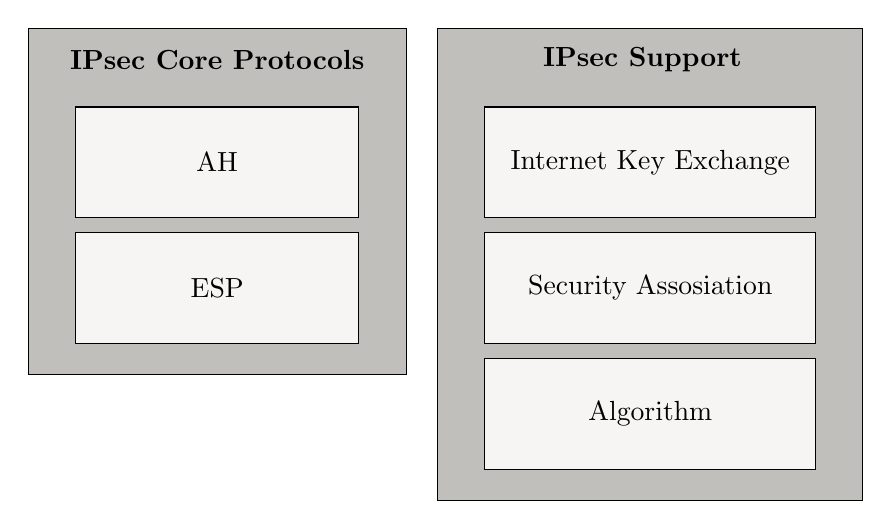
\begin{tikzpicture}[scale=0.8]
            \draw [ fill={rgb,255:red,192;green,191; blue,188} ] (5.5,13.25) rectangle (11.5,7.75); 
            \draw [ fill={rgb,255:red,246;green,245; blue,244} ] (6.25,10) rectangle node {ESP} (10.75,8.25); 
            \draw [ fill={rgb,255:red,192; green,191; blue,188} ] (12,13.25) rectangle (18.75,5.75); 
            \draw [ fill={rgb,255:red,246; green,245; blue,244} ] (6.25,12) rectangle node {AH} (10.75,10.25); 
            \node at (8.5,12.75) {\textbf{IPsec Core Protocols}}; 
            \node at (15.25,12.75) {\textbf{IPsec Support}}; 
            \draw [ fill={rgb,255:red,246; green,245; blue,244} ] (12.75,12) rectangle node { Internet Key Exchange} (18,10.25); 
            \draw [ fill={rgb,255:red,246; green,245; blue,244} ] (12.75,10) rectangle node { Security Assosiation} (18,8.25); 
            \draw [ fill={rgb,255:red,246; green,245; blue,244} ] (12.75,8) rectangle node { Algorithm} (18,6.25); 
        \end{tikzpicture}
    }
\label{fig:ipsec-suite} 
\caption{IPsec Protolocol Suite}
\end{figure}
\subsection{Security Association}

Le comunicazioni sicure si costruiscono sopra un concetto fondamentale noto come Security Association (SA). 



\subsection{IKE}


Il protocollo IKEv2, definito nell'\texttt{RFC 7296}, è un protocollo di rete che è responsabile della negoziazione di chiavi crittografiche e dei parametri di sicurezza tra due dispositivi, solitamente chiamati peer.

\begin{figure}[htbp]
    \centering
    \begin{tikzpicture}[node distance=1.5cm]
        % Initiator and Responder
        \node (entity1) [draw=red, rectangle] {Initiator (\textit{i})};
        \node (entity2) [draw=blue, rectangle, right=of entity1, xshift=3cm] {Responder (\textit{r})};
        \draw (entity1) -- ++(0,-6.7) coordinate (vertical1);
        \draw (entity2) -- ++(0,-6.7);
        % IKE_INIT_SA
        \draw[-stealth] (entity1) ++(0,-1) -- (entity2 |-,-1) node[midway, above, text=red, font=\footnotesize] {$SA_{i1}, KE_i, N_i$};
        \draw[stealth-] (entity1) ++(0,-2) -- (entity2 |-,-2) node[midway, above, text=blue, font=\footnotesize] {$SA_{r1},KE_r,N_r$};
        % IKE_AUTH
        \draw[-stealth] (entity1) ++(0,-3.5) -- (entity2 |-,-3.5) node[midway, above, text=red, font=\footnotesize] {$SK\{ID_i, CERT, \{AUTH\}^s_{pk}\}$};
        \draw[stealth-] (entity1) ++(0,-4.5) -- (entity2 |-,-4.5) node[midway, above, text=blue, font=\footnotesize] {$SK\{ID_r, CERT, \{AUTH\}^s_{pk}\}$};
        % CHILD_SA 
        \node at (-1.7,-6) {\inlinecode{CHILD\_SA}};
        \node at (-2,-1.5) {\inlinecode{IKE\_SA\_INIT}};
        \node at (-1.7,-4) {\inlinecode{IKE\_AUTH}};
        \draw (entity1) ++(0.2,-6) ellipse (0.2cm and 0.2cm);
        \draw [-] (0.2,-6.2) -- (6.65,-6.2);
        \draw [-] (0.2,-5.8) -- (6.65,-5.8) node[midway, above, font=\footnotesize]{$SK_d, N_i, N_r$};
        \draw (entity2) ++(-0.2,-6) ellipse (0.2cm and 0.2cm);
        % Key for encryption and authtenticatoin
        \drawkey{-1, -2.3}{red}{$SK_{ei}$};
        \drawkey{-1.8, -2.3}{red}{$SK_{ai}$};
        \drawkey{8, -2.3}{blue}{$SK_{ar}$};
        \drawkey{8.8, -2.3}{blue}{$SK_{er}$};
        % Group
        \drawcurlybrace{0,-1}{0, -2}{};
        \drawcurlybrace{0,-3.5}{0, -4.5}{};
    \end{tikzpicture}
    \label{fig:ike_exchange}
    \caption{Fasi di Negoziazione del Protocollo IKEv2}
\end{figure}

Lo schema generale di funzionamento del protocollo al termine del quale i due hanno stabilito una SA è riportato in \textit{Fig. \ref{fig:ike_exchange}}.

\subsection{\textbf{IKE\_SA\_INIT}}

Lo scopo di questa prima fase è quello di creare una \textbf{IKE SA}, che consenta di rendere sicure i successivi scambi di dati al fine di realizzare una \textbf{IPsec SA}.
Dunque funge da apripista al fine di stabilire quelli che sono i parametri di sicurezza al fine di avere una comunicazione sicura. Per questo motivo in questo scambio i peer 
si scambiano le seguenti informazioni:

\begin{table}[htbp]
    \centering
    \caption{Tabella dei parametri e delle descrizioni}
    \begin{tabular}{ll}
        \toprule
        \textbf{Parametro} & \textbf{Descrizione} \\
        \midrule
        \textit{SA} & Security Association, vengono negoziati i parametri per la SA\\
        \textit{KE} & Key Exchange, e nel caso classico è l'esponente DH \\
        \textit{N} & Nonce \\
    \bottomrule
    \end{tabular}
\end{table}

\noindent
Al termine di questo scambio i due peer ottengono il \textit{DH Shared Secret} (indicato con $g^{ir}$), il quale insisme ai nonce, consentirà di ottenere 
quelli che sono i parametri di sicurezza della $IKE SA$ al fine di instauare un canale sicuro, per approfondimenti in \href{AppendixA}{appendice}.

% Tabella che riporta le varie funzioni delle chiavi

\subsection{IKE\_AUTH}

Il risultato della fase precedente è un canale sicuro su cui comunicare, in quanto è cifrato e utenticato. Si questo hanno luogo gli scambi per instaurare la IPsec SA.
In questa fase i nodi si autenticano mutuamente:

\begin{table}[htbp]
    \centering
    \caption{Tabella dei parametri e delle descrizioni}
    \begin{tabular}{ll}
        \toprule
        \textbf{Parametro} & \textbf{Descrizione} \\
        \midrule
        \textit{AUTH} & Payload che deve essere firmato affinchè ci sia autenticazione \\
        \textit{CERT} & Si allega il certificato digitale per la chiave pubblica \\
        \textit{CERTQ} & Si fa richiesta al peer di fornire il certificato \\
    \bottomrule
    \end{tabular}
\end{table}

Tutto il contenuto appena descritto è protetto mediante le chiavi segrete di quella direzione. Ciò è indicato mediante la notazione $SK\{...\}$
La modalità di autenticazione può essere: PSK, EAP oppure mediante chiave pubblica.

\subsection{CHILD\_SA}


\section{Problemi}

IKEv2 utilizza come porotocollo a livello trasporto UDP per per inoltrare i propri messaggi. La maggior parte dei messaggi che i peer si scambiano hanno dimensioni relativamente piccole e
quindi che non eccedono l'\textbf{MTU} di un pacchetto IP, tuttavia abbiamo degli scambi che richiedono un trasferimento di dati abbastanza grandi.

Per esempio nel caso di autenticazione tramite pubkey nella fase di \inlinecode{IKE\_AUTH} è necessario trasferire il proprio certificato che in base allo schema di firma utilizzato
può arrivare anche a diversi Kbyte di dimensione. In questi casi si verifica la frammentazione a livello IP.

%Immagine frammentazione

\begin{figure}[htbp]
    \centering
    \begin{tikzpicture}[node distance=2cm,>=Latex]
        % Nodi
        \node (initiator) [client] {Initiator};
        \node (device) [router, right=of initiator] {Device};
        \node (responder) [client, right=of device] {Responder};
        \node (message) [messageclosed, fill=orange!40, minimum size=0.6cm] at (1.9,0.5) {};
        \node (message2) [messageclosed, fill=gray!40, minimum size=0.6cm] at (1.2,0.5) {};
        \node (drop) [messageclosed, fill=gray!40, minimum size=0.6cm, , font=\small, text=red] at (3,1) {};
        \node (message3) [messageclosed, fill=orange!40, minimum size=0.6cm, , font=\small, text=red] at (4.5,0.5) {};

        \draw[-] (initiator.east) -- (device.west);
        \draw[-] (device.east) -- (responder.west);

    \end{tikzpicture}
    \vspace*{1cm}
    \caption{Drop Pacchetti}
    \label{fig:cgnatdrop}
\end{figure}

Diversi test hanno mostrato che nel caso in cui i peer si trovino in presenza di CGNAT potrebbero non istausarsi le SA. Questo è dovuto al fatto che i device degli ISP non
consentono ai frammenti IP di passare attravers di loro, ovvero scartano i pacchetti e di conseguenza bloccano le comunicazioni IKE.
Questo è riportato schematicamente in Fig. \ref{fig:cgnatdrop}.
Questo drop dei pacchetti avviene perchè esistono numerosi vettori di attacco che fanno affidamento sulla frammentazione IP, per questo motivo gli ISP operano un filtro su questa tipologia di pacchetti.
Ance se in teoria uno dei requisiti del CGNAT definito dagli RFC è proprio consentire la frammentazione.

Per risolvere questa problematica e dunque consentire il passaggio dei messaggi attraverso i dispositivi di rete che non consentono il passaggio degli IP fragment attraverso 
di loro nell' RFC 7283 viene introdotta la IKEv2 \textit{Message Fragmentation}. In cui la frammentazione dei messaggi è gestita direttamente da parte di chi implementa IKEv2

\subsection{\inlinecode{IKE\_INTERMEDIATE}}

Per evitare che nel trasferimento di grandi dati ciò avvenga viene introdotto uno scambio aggiuntivo. Questo scambio è introdotto per quei casi in cui la dimensione dei dati
da trasferire ecceda la dimensione massima che causerebbe la frammentazione IP. Questo scambio va fatto dopo la \inlinecode{IKE\_INIT\_SA} e prima della \inlinecode{IKE\_AUTH} in questo
modo è sia autenticato che cifrato tramite le chiavi negoziate dal primo scambio.

\begin{figure}[htbp]
    \centering
    \begin{tikzpicture}[node distance=1.5cm]
        % Initiator and Responder
        \node (entity1) [draw=red, rectangle] {Initiator (\textit{i})};
        \node (entity2) [draw=blue, rectangle, right=of entity1, xshift=3cm] {Responder (\textit{r})};
        \draw (entity1) -- ++(0,-4.5) coordinate (vertical1);
        \draw (entity2) -- ++(0,-4.5);
        % IKE_AUTH
        \draw[stealth-stealth] (entity1) ++(0,-1.5) -- (entity2 |-,-1.5) node[midway, above] {\inlinecode{IKE\_SA\_INIT}};
        \draw[stealth-stealth] (entity1) ++(0,-2.5) -- (entity2 |-,-2.5) node[midway, above] {[\inlinecode{IKE\_INTERMEDIATE}]};
        \draw[stealth-stealth] (entity1) ++(0,-3.5) -- (entity2 |-,-3.5) node[midway, above] {\inlinecode{IKE\_AUTH}};
    \end{tikzpicture}
    \caption{Scambio nuovo}
    \label{fig:ikeintermediate}
\end{figure}

Questo scambio è posizionato qui in quanto nella \inlinecode{IKE\_SA\_INIT} per motivi di sicurezza non è possibile applicare la frammentazione.
Di solito i messaggi sono piccoli abbastanza da non causare la frammentazione IP, tuttavia questo potrebbe cambiare se si utilizzano scambi di chiave QC-resistant; in quanto
hanno chiavi pubbliche larghe e che quindi causerebbero frammentazione IP.

Per questo viene aggiunto questo scambio che viene utilizzato per trasferire grandi quantità di dati.

L'utilizzo principale di questo scambio è quello di trasferire le chiavi pubbliche QC-resistant, tuttavia in generale può essere utilizzzato per trasferire qualsiasi tipologia di dato.
Quindi il principale utilizzo è quello di fare un \textbf{enforcing} delle chiavi negoziate tramite DH al fine di renderle QC-resistant. Infatti se durante questo scambio si scambiano 
altre chiavi allora le coppie $\{SK_{a[i/r]}, SK_{e[i/r]}\}$ vengono aggiornate.

Permette di realizzare Multiple Key Exchange
Gli scambi di chiave aggiuntivi vengono aggiunti alla proposal tramite \inlinecode{PQ\_KEM\_1}



Lo scambio \inlinecode{IKE\_FOLLOWUP\_KE} è introdotto specificatamente per trasferire dati sulla chiavi addizionali da realizzare in una CHILD SA.
In questo caso le chiavi aggiuntive vengono utilizzate per aggiornare il KEYMAT



\begin{itemize}
    \item flag \inlinecode{IKE\_FRAGMENTATION\_SUPPORT}: il peer dice di supportare la frammentazione IKEv2, affinchè venga utilizzata entrambi i peer devono supportarla.
    \item flag \inlinecode{INTERMEDIATE\_EXCHANGE\_SUPPORT}: il peer dice di supportare gli scambi intermedi
\end{itemize}

Una volta terminati gli scambi, per proteggere lo scambio \inlinecode{IKE\_AUTH} e gli scambi successivi vengno utilizzata le ultime chiavi calcolate
Dato che i dati trasferiti in questi scambi aggiuntivi vanno autenticati si aggiungono all'\inlinecode{AUTH} payload che poi andrà 



Il supporto per lo scambio aggiuntivo viene comunicato aggiungendo all'interno
dell \inlinecode{IKE\_SA\_INIT} il flag \inlinecode{IKE\_INT\_SUP} (che sta per
Intermediate Exchange Support).
Se anche il responder lo supporta lo includerà nel messaggio di risposta dello
scambio.




Considerazioni, L'IKE fragmentation viene introdotta a causa del NAT tuttavia nel nostro caso di satelliti non ha senso utilizzarla in quanto non credo che si utilizzi
il NAT soprattutto perchè introduce ritardi dovuti alla traduzione degli indirizzi



\section{Post-Quantum}

Un solo KEM con Kyber L1 usando come suite AES\_GCM has vabene come certificato dilithium L1

Nel KEM quanti cifrano?

Cioè l'initiator manda il certificato e poi il responder cifra 
